% 2009 年广东卷（文科）第 1 题：四个韦恩（Venn）图选项。
% 来源 PDF：.work/ocr-local/sources/2009广东文.pdf
% SHA-256：26c26718ce8f1cd1128fca4e63e1576ecec72ee27cc46ad538673bb533e61ced
% 原页：第 1 页（A3 三栏）第 1 栏，印刷页 521。
% 绘制依据：矩形表示全集 U；原页四个选项的图内位置与包含关系为
%   (A) 左圆 N、右圆 M 相交且各有外露部分；
%   (B) 小圆 N 含于大圆 M 内（M 为大圆）；
%   (C) 圆 M 在左、圆 N 在右，互不相交；
%   (D) 小圆 M 含于大圆 N 内（N 为大圆）。
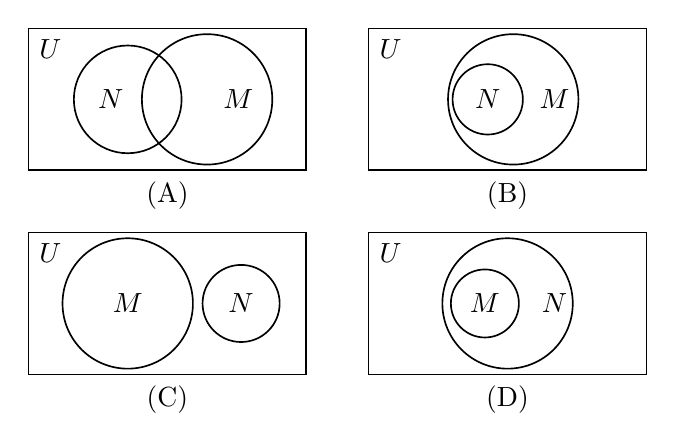
\begin{tikzpicture}[scale=0.72, semithick, every node/.style={inner sep=2pt}]

  % ---------------- (A) N 与 M 相交 ----------------
  \begin{scope}
    \draw (0,0) rectangle (4.9,2.5);
    \node[anchor=north west] at (0.08,2.42) {$U$};
    \draw (1.75,1.25) circle (0.95);
    \draw (3.15,1.25) circle (1.15);
    \node at (1.45,1.25) {$N$};
    \node at (3.70,1.25) {$M$};
    \node at (2.45,-0.45) {(A)};
  \end{scope}

  % ---------------- (B) N 含于 M 内 ----------------
  \begin{scope}[shift={(6.0,0)}]
    \draw (0,0) rectangle (4.9,2.5);
    \node[anchor=north west] at (0.08,2.42) {$U$};
    \draw (2.55,1.25) circle (1.15);
    \draw (2.10,1.25) circle (0.62);
    \node at (2.10,1.25) {$N$};
    \node at (3.28,1.25) {$M$};
    \node at (2.45,-0.45) {(B)};
  \end{scope}

  % ---------------- (C) M 与 N 互不相交 ----------------
  \begin{scope}[shift={(0,-3.6)}]
    \draw (0,0) rectangle (4.9,2.5);
    \node[anchor=north west] at (0.08,2.42) {$U$};
    \draw (1.75,1.25) circle (1.15);
    \draw (3.75,1.25) circle (0.68);
    \node at (1.75,1.25) {$M$};
    \node at (3.75,1.25) {$N$};
    \node at (2.45,-0.45) {(C)};
  \end{scope}

  % ---------------- (D) M 含于 N 内 ----------------
  \begin{scope}[shift={(6.0,-3.6)}]
    \draw (0,0) rectangle (4.9,2.5);
    \node[anchor=north west] at (0.08,2.42) {$U$};
    \draw (2.45,1.25) circle (1.15);
    \draw (2.05,1.25) circle (0.60);
    \node at (2.05,1.25) {$M$};
    \node at (3.28,1.25) {$N$};
    \node at (2.45,-0.45) {(D)};
  \end{scope}

\end{tikzpicture}
